\chapter[Resultados]{Resultados}

%4. Resultados da Revisão Sistemática
%Aqui você apresentará os achados consolidados dos estudos selecionados, organizados para responder diretamente às suas questões de pesquisa. Sugiro dividir em subseções temáticas, conforme as perguntas:

Este capítulo apresenta a síntese dos achados da revisão sistemática de literatura, organizados para responder às questões de pesquisa definidas no estudo. A partir da análise dos 25 estudos selecionados (conforme detalhado no Capítulo 3), foram identificados padrões, técnicas, ferramentas e contextos associados à prototipação em DS.

Inicialmente, são descritas as principais técnicas de prototipação utilizadas no DS, seguidas de uma caracterização de seus objetivos, métodos e resultados esperados. Em seguida, é explorada a aplicabilidade dessas técnicas em diferentes contextos e etapas do processo de DS, como ideação, validação ou implementação. Além disso, são apresentadas as ferramentas mais recorrentes na literatura, comparando-as em termos de funcionalidades e adequação às necessidades do projeto. Por fim, discute-se o fluxo do processo de prototipação, destacando as entradas necessárias (ex.: dados de usuários, requisitos) e as saídas geradas (ex.: protótipos iterativos, insights de validação).

A análise foi conduzida como planejado no protocolo. Para facilitar a visualização foram utilizadas tabelas comparativas e diagramas. Logo abaixo, segue uma tabela indicando quais questões da pesquisa cada estudo selecionado responde.

\begin{table}[h!]
	\centering
	\label{tab:triagem}
	\begin{tabular}{|c|c|c|c|c|c|c|c|}
		\hline
		\textbf{ID} & \textbf{Referência} & \textbf{Q1} & \textbf{Q2} & \textbf{Q3} & \textbf{Q4} & \textbf{Q5} & \textbf{Q6} \\ \hline
		E1 & \cite{asbjornsen2022echange} & \checkmark & \checkmark & \checkmark & \checkmark & \checkmark & \checkmark \\ \hline
		E2 & \cite{dehmel2021weather} & \checkmark & \checkmark & \checkmark & x & x & \checkmark \\ \hline
		E3 & \cite{giraldo2024ecotourism} & \checkmark & \checkmark & \checkmark & x & x & \checkmark \\ \hline
		E4 & \cite{kumar2023rheumatology} & \checkmark & \checkmark & \checkmark & \checkmark & \checkmark & \checkmark \\ \hline
		E5 & \cite{lambe2022capabilities} & \checkmark & \checkmark & \checkmark & x & x & \checkmark \\ \hline
		E6 & \cite{lee2023industry} & \checkmark & \checkmark & \checkmark & \checkmark & \checkmark & \checkmark \\ \hline
		E7 & \cite{milton2021eatingdisorders} & \checkmark & \checkmark & \checkmark & x & x & \checkmark \\ \hline
		E8 & \cite{seko2024transitions} & \checkmark & \checkmark & \checkmark & \checkmark & \checkmark & \checkmark\\ \hline
		E9 & \cite{soto2023prototyping} & \checkmark & \checkmark & \checkmark & \checkmark & \checkmark & \checkmark\\ \hline
		E10 & \cite{villa2022integratedcare} & \checkmark & \checkmark & \checkmark & \checkmark & \checkmark & \checkmark \\ \hline
		E11 & \cite{wang2023smartproducts} & \checkmark & \checkmark & \checkmark & \checkmark & \checkmark & \checkmark \\ \hline
		E12 & \cite{yan2022pssvalue} & \checkmark & \checkmark & \checkmark & \checkmark & \checkmark & \checkmark\\ \hline
		E13 & \cite{Kim2024} & \checkmark & \checkmark & x & \checkmark & \checkmark & \checkmark\\ \hline
		E14 & \cite{Suryawati2024} & \checkmark & \checkmark & \checkmark & x & \checkmark & \checkmark\\ \hline
		E15 & \cite{hegemann2024palette} & \checkmark & \checkmark & \checkmark & \checkmark & \checkmark & \checkmark\\ \hline
		E16 & \cite{lee2022how} & \checkmark & x & x & x & x & x\\ \hline
		E17 & \cite{quintero2021interdisciplinary} & \checkmark & \checkmark & \checkmark & \checkmark & x & \checkmark \\ \hline
		E18 & \cite{iriarte2023service} & \checkmark & \checkmark & \checkmark & x & x & \checkmark \\ \hline
		E19 & \cite{leinonen2023service} & \checkmark & x & \checkmark & x & x & \checkmark\\ \hline
		E20 & \cite{mager2023product} & \checkmark & \checkmark & \checkmark & \checkmark & \checkmark & \checkmark\\ \hline
		E21 & \cite{nguyen2022human} & \checkmark & \checkmark & \checkmark & x & x & \checkmark\\ \hline
		E22 & \cite{paust2025integrative} & \checkmark & \checkmark & \checkmark & \checkmark & \checkmark & \checkmark\\ \hline
		E23 & \cite{Vieira2025} & \checkmark & \checkmark & \checkmark & x & \checkmark & \checkmark\\ \hline
		E24 & \cite{schlott2024design} & \checkmark & \checkmark & \checkmark & x & x & \checkmark\\ \hline
		E25 & \cite{you2022applying} & \checkmark & \checkmark & x & x & x & \checkmark \\ \hline

	\end{tabular}
	\caption{Relação dos estudos com as questões de pesquisa}
\end{table}

%4.1 Principais técnicas de prototipação em Design de Serviços
%Liste e descreva as técnicas identificadas (ex.: storyboards, service blueprints, role-playing, protótipos físicos/digitais, cenários, simulações).

%Inclua uma tabela comparativa (técnica, autores, definição).

\section{Principais técnicas de prototipação em Design de Serviços}

A primeira questão dessa revisão sistemática de literatura buscou identificar as principais técnicas de prototipagem empregadas no contexto do DS, conforme abordado nos 25 artigos selecionados. A análise demonstrou diferentes tipos de técnicas, refletindo a natureza diversificada dos serviços e a necessidade de representar diferentes aspectos da experiência, do processo e dos pontos de contato. Essas técnicas variam consideravelmente em termos de fidelidade (baixa, média, alta), formato (físico, digital, conceitual, experiencial) e propósito principal (exploração, comunicação, teste, validação).

Para organizar a diversidade encontrada, as técnicas identificadas foram agrupadas nas seguintes categorias principais: (1) Prototipagem Conceitual e Visual; (2) Prototipagem Experiencial e de Interação; (3) Prototipagem Física e Tangível; (4) Prototipagem Digital e Funcional; e (5) Prototipagem Estratégica e Holística.


\begin{comment}
\begin{figure}
	\centering
	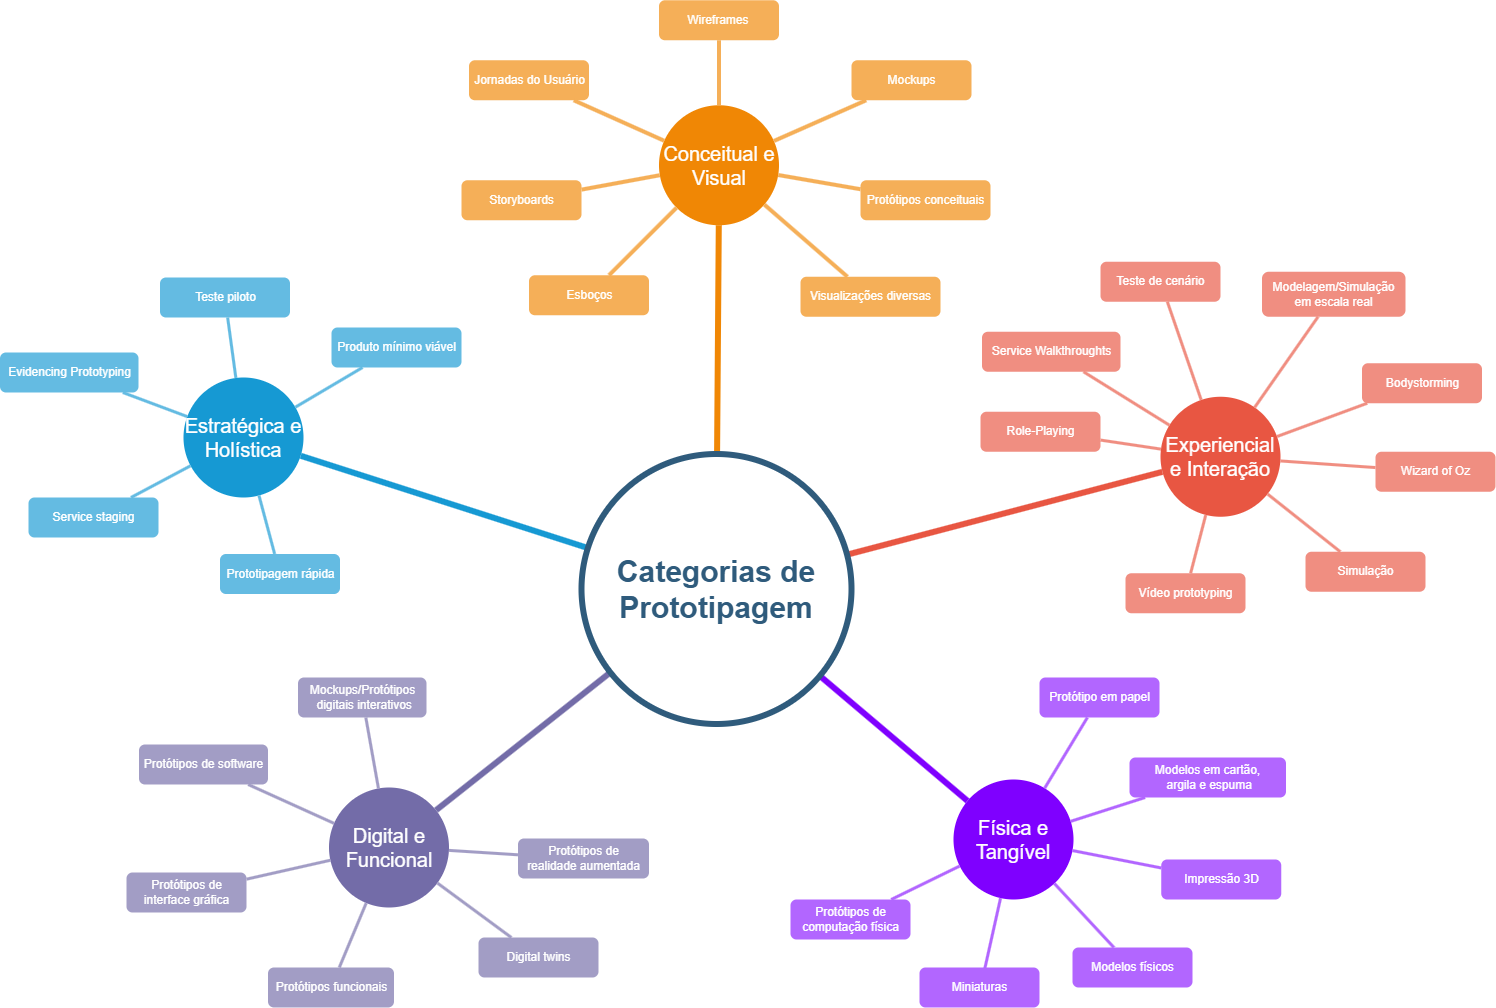
\includegraphics[width=1\linewidth]{figuras/categorias-prototipacao}
	\caption{Categaorias da prototipação}
	\label{fig:categorias-prototipacao}
\end{figure}
\end{comment}

\subsection{Prototipagem conceitual e visual}

Nessa categoria de prototipagem, as técnicas tem como objetivo principal externalizar, comunicar e refinar ideias mais abstratas, fluxos de serviço, jornadas do usuário e conceitos inciais, na maior parte dos casos não serão protótipos de alta fidelidade. Abaixo são listadas as principais técnicas dessa categoria, além dos estudos que abordaram cada uma das técnicas.

\begin{itemize}
	\item \textbf{Esboços}: Desenhos rápidos, tanto manuais como digitais, para explorar formas e ideias iniciais. Os seguintes estudos abordaram sobre essa técnica: \citeonline{hegemann2024palette, nguyen2022human, paust2025integrative, kumar2023rheumatology, Suryawati2024, wang2023smartproducts, lambe2022capabilities}.
	
	\item \textbf{Storyboards e animações}: Sequências visuais que narram uma interação ou jornada de serviço. Os seguintes estudos abordaram sobre essa técnica: \citeonline{lee2022how, mager2023product, paust2025integrative, wang2023smartproducts, lee2023industry}.
	
	\item \textbf{Jornadas do usuário e mapas de experiência}: Visualizações que mapeiam os passos, emoções e pontos de contato do usuário ao longo do serviço. Os seguintes estudos abordaram sobre essa técnica: \citeonline{mager2023product, paust2025integrative, milton2021eatingdisorders, wang2023smartproducts}.
	
	\item \textbf{\textit{Wireframes} e \textit{Mockups}}: Representações estruturais (wireframes) ou visuais (mockups) de interfaces digitais ou \textit{layouts}, em papel ou software, normalmente em baixa ou média fidelidade. Os seguintes estudos abordaram sobre essa técnica: \citeonline{hegemann2024palette, lee2022how, leinonen2023service, nguyen2022human, paust2025integrative, asbjornsen2022echange, milton2021eatingdisorders, villa2022integratedcare, Suryawati2024, wang2023smartproducts, Kim2024}.
	
	\item \textbf{Protótipos conceituais}: Descrições, diagramas ou modelos simplificados que representam a lógica ou a estrutura de uma intervenção, serviço ou modelo de negócio, frequentemente usados como ``material gatilho'' para discussão. Os seguintes estudos abordaram sobre essa técnica: \citeonline{you2022applying, dehmel2021weather, lambe2022capabilities, yan2022pssvalue}.
	
	\item \textbf{Visualizações diversas}: Incluindo ilustrações, canvas (como \textit{Business Model} Canvas), diagramas, \textit{pitch decks}, etc., usados para comunicar conceitos. Os seguintes estudos abordaram sobre essa técnica: \citeonline{paust2025integrative, you2022applying}.
	
	\item \textbf{Artefatos descritivos e \textit{mood boards}}: Coleções de elementos visuais ou textuais para comunicar a estética, o tom ou componentes específicos do serviço. Os seguintes estudos abordaram sobre essa técnica: \citeonline{hegemann2024palette, milton2021eatingdisorders}.
\end{itemize}

\subsection{Prototipagem experiencial e de interação}

Essenciais para o DS devido à natureza experiencial e co-criada dos serviços, estas técnicas buscam simular a interação humana, o fluxo do serviço e a experiência vivida pelos usuários. Incluem:

\begin{itemize}
	\item \textbf{\textit{Role-Playing} e Encenação}: Participantes assumem papéis (clientes, funcionários) para encenar interações e cenários de serviço. Os seguintes estudos abordaram sobre essa técnica: \citeonline{lee2022how, iriarte2023service, mager2023product, paust2025integrative, Vieira2025, kumar2023rheumatology, seko2024transitions, soto2023prototyping}.
	
	\item \textbf{\textit{Service Walkthroughs / Desktop Walkthroughs}}: Simulações passo a passo do processo de serviço, seja em um ambiente físico simulado ou usando representações em uma mesa. Os seguintes estudos abordaram sobre essa técnica: \citeonline{iriarte2023service, mager2023product, seko2024transitions}.
	
	\item \textbf{Teste de cenários}: Uso de cenários específicos para guiar a interação dentro de um protótipo (frequentemente experiencial). Os seguintes estudos abordaram sobre essa técnica: \citeonline{seko2024transitions, soto2023prototyping}.
	
	\item \textbf{Modelagem/Simulação em Escala Real}: Representações estruturais (wireframes) ou visuais (mockups) de interfaces digitais ou \textit{layouts}, em papel ou software, normalmente em baixa ou média fidelidade. Os seguintes estudos abordaram sobre essa técnica: \citeonline{seko2024transitions, soto2023prototyping, yan2022pssvalue}.
	
	\item \textbf{\textit{Bodystorming}}: Exploração de ideias e experiências usando o corpo e o espaço físico. O seguinte estudo abordou sobre essa técnica: \citeonline{Kim2024}.
	
	\item \textbf{\textit{Wizard of Oz}}: Técnica onde um usuário interage com um sistema que parece autônomo, mas é secretamente operado por um humano (``mágico'') para simular funcionalidades futuras. Os seguintes estudos abordaram sobre essa técnica: \citeonline{lee2022how, Kim2024}.
	
	\item \textbf{Simulação\textit{``concierge''}}: Simulação interna, manual, de um serviço (geralmente digital) pela equipe para identificar falhas antes do desenvolvimento. O seguinte estudo abordou sobre essa técnica: \citeonline{Suryawati2024}.
\end{itemize}

\subsection{Prototipagem Física e Tangível}

Aqui, é envolvida a criação de artefatos físicos que representam produtos associados ao serviço, pontos de contato tangíveis ou elementos usados em simulações. Exemplos:

\begin{itemize}
	\item \textbf{Protótipos em papel}:  Incluindo interfaces, formulários ou outros elementos impressos para teste rápido. Os seguintes estudos abordaram sobre essa técnica: \citeonline{lee2022how, nguyen2022human, asbjornsen2022echange, Kim2024}.
	
	\item \textbf{Modelos em cartão, argila e espuma}: Usados para explorar formas físicas ou construir representações em simulações. Os seguintes estudos abordaram sobre essa técnica: \citeonline{wang2023smartproducts, lee2023industry}.
	
	\item \textbf{Impressão 3D}: Utilizada para criar objetos físicos com maior precisão. Os seguintes estudos abordaram sobre essa técnica: \citeonline{quintero2021interdisciplinary, wang2023smartproducts}.
	
	\item \textbf{Modelos Físicos (em escala ou 1:1)}: Representações de produtos ou ambientes. Os seguintes estudos abordaram sobre essa técnica: \citeonline{mager2023product, paust2025integrative, nguyen2022human, lee2023industry, yan2022pssvalue}.
	
	\item \textbf{Miniaturas, materiais de artesanato e fantasias}:Usados de forma criativa em prototipagem de baixa fidelidade ou simulações. Os seguintes estudos abordaram sobre essa técnica: \citeonline{lee2023industry, seko2024transitions}.
	
	\item \textbf{Elementos tangíveis}: Itens físicos que fazem parte do serviço (ex: guias impressos, \textit{``swag-bags'')}. O seguinte estudo abordou sobre essa técnica: \citeonline{kumar2023rheumatology}.
	
	\item \textbf{Protótipos de computação física (IoT)}: Envolvem hardware (sensores, atuadores, microcontroladores como Arduino, ESPBoost) para criar sistemas interativos. O seguinte estudo abordou sobre essa técnica: \citeonline{Kim2024}.
\end{itemize}

\subsection{Prototipagem digital e funcional}

Com a crescente digitalização dos serviços, técnicas para prototipar interfaces e funcionalidades digitais são cruciais. Incluem:

\begin{itemize}
	\item \textbf{\textit{Mockups}/Protótipos Digitais Interativos}:  Criados com softwares específicos (ex: Figma, Marvel), variando de baixa a alta fidelidade, permitindo simular a navegação e interação. Os seguintes estudos abordaram sobre essa técnica: \citeonline{lee2022how, asbjornsen2022echange, giraldo2024ecotourism, kumar2023rheumatology, lee2023industry, villa2022integratedcare, Kim2024}.
	
	\item \textbf{Protótipos de software}: Versões iniciais e funcionais de um software ou aplicativo. Os seguintes estudos abordaram sobre essa técnica: \citeonline{leinonen2023service, nguyen2022human}.
	
	\item \textbf{Protótipos de Interface Gráfica (GUI)}: Focados no design visual e funcional da interface. O seguinte estudo abordou sobre essa técnica: \citeonline{nguyen2022human}.
	
	\item \textbf{Protótipos Funcionais (\textit{Working Prototypes} - IoT)}: Sistemas que demonstram a funcionalidade central de um serviço IoT, integrando \textit{hardware}, \textit{software} e rede. O seguinte estudo abordou sobre essa técnica: \citeonline{Kim2024}.
	
	\item \textbf{\textit{Digital twins}}: Representações digitais dinâmicas de sistemas ou processos físicos. O seguinte estudo abordou sobre essa técnica: \citeonline{mager2023product}.
	
	\item \textbf{Protótipos de Realidade Aumentada (AR) / Realidade Virtual (VR)}: Uso de tecnologias imersivas para simular ou complementar a experiência de serviço. Os seguintes estudos abordaram sobre essa técnica: \citeonline{lee2022how, wang2023smartproducts, giraldo2024ecotourism}.
\end{itemize}

\subsection{Prototipagem estratégica e holística}

Algumas abordagens ou resultados da prototipagem têm um caráter mais amplo, estratégico ou de teste em condições reais:

\begin{itemize}
	\item \textbf{Produto Mínimo Viável}: Versão simplificada do serviço lançada para testar hipóteses fundamentais no mercado real. Os seguintes estudos abordaram sobre essa técnica: \citeonline{paust2025integrative, giraldo2024ecotourism}.
	
	\item \textbf{Teste piloto}: Implementação do serviço em pequena escala, em um contexto real, como forma de prototipagem viva ou teste final. O seguinte estudo abordou sobre essa técnica: \citeonline{seko2024transitions}.
	
	\item \textbf{\textit{Evidencing prototyping}}: Criação de artefatos que servem como ``evidência'' tangível de pontos de contato, mesmo os menos óbvios (ex: rascunhos de contratos, materiais de marketing, relatórios técnicos). O seguinte estudo abordou sobre essa técnica: \citeonline{iriarte2023service}.
	
	\item \textbf{\textit{Service staging}}: Conceito relacionado à montagem de um ambiente e processo para simular a entrega do serviço, próximo da simulação em escala real. O seguinte estudo abordou sobre essa técnica: \citeonline{lee2022how}.
	
	\item \textbf{Prototipagem rápida}: Uma abordagem ou filosofia que enfatiza a criação rápida de protótipos (geralmente de baixa fidelidade) para aprendizado e iteração ágil. Os seguintes estudos abordaram sobre essa técnica: \citeonline{paust2025integrative, you2022applying, asbjornsen2022echange, dehmel2021weather}.
\end{itemize}

%4.2 Caracterização das técnicas
%Analise os objetivos (ex.: testar interações, validar fluxos de serviço), métodos (como são aplicadas) e resultados esperados (ex.: insights sobre experiência do usuário, validação de processos).

%Use exemplos dos estudos para ilustrar.

\section{Caracterização das técnicas de prototipagem em relação aos objetivos, métodos e resultados}

A análise dos estudos selecionados permitiu a caracterização das diversas técnicas de prototipagem que foram identificadas na seção anterior, em termos de seus objetivos, métodos empregados e resultados esperados no contexto do DS. A caracterização revela que a prototipagem em DS ultrapassa a simples criação de modelos para teste, assumindo múltiplas funções ao longo do processo de design.

\subsection{Objetivos da prototipagem em DS}

Os artigos de forma geral, indicam uma variedade de propósitos ao utilizar a prototipagem no DS. Esses propósitos podem ser agrupados em grupos, sendo eles: \textbf{Comunicação} e \textbf{compreensão}, \textbf{exploração} e \textbf{aprendizagem}, \textbf{avaliação} e \textbf{refinamento}, \textbf{concretização} e \textbf{tomada de decisões}, \textbf{empatia} e \textbf{engajamento}.

Inicialmente, a \textbf{comunicação} e \textbf{compreensão} são focos centrais, pois um objetivo fundamental é tornar ideias abstratas tangíveis e visíveis para facilitar a comunicação e construir um entendimento compartilhado entre membros da equipe e \textit{stakeholders} \cite{paust2025integrative, mager2023product, soto2023prototyping, lee2023industry}. Isso inclui explicar conceitos, visualizar fluxos e jornadas, além de ultrapassar barreiras de linguagem entre disciplinas \cite{paust2025integrative, wang2023smartproducts}.

Em relação a \textbf{exploração} e \textbf{aprendizagem}, a prototipagem serve como ferramenta de exploração para investigar o problema e a solução, aprender sobre as necessidades e o contexto dos usuários, identificar novas oportunidades e gerar alternativas \cite{paust2025integrative, mager2023product, soto2023prototyping, you2022applying, dehmel2021weather, lambe2022capabilities}. A aprendizagem por tentativa e erro, incluindo falhas de baixo custo, é frequentemente destacada \cite{paust2025integrative, soto2023prototyping, you2022applying}.

Já a \textbf{avaliação} e \textbf{refinamento}, vem para testar conceitos, validar suposições, avaliar usabilidade e viabilidade, obter feedback de usuários e stakeholders, além de refinar iterativamente as soluções, são objetivos clássicos da prototipagem, também presentes no DS \cite{paust2025integrative, hegemann2024palette, quintero2021interdisciplinary, mager2023product, Vieira2025, asbjornsen2022echange, villa2022integratedcare}. Isso inclui prever e prevenir falhas na experiência \cite{mager2023product}.

No quesito da \textbf{concretização} e \textbf{tomada de decisões}, é válido ressaltar a importância de converter ideias em formas tangíveis para permitir decisões mais informadas, selecionar as melhores alternativas, definir o escopo, criar MVPs e informar a implementação final são funções importantes \cite{nguyen2022human, Vieira2025, schlott2024design, quintero2021interdisciplinary, iriarte2023service}.

Por último, a \textbf{empatia} e \textbf{engajamento} fazem com que a prototipagem, especialmente a experiencial, busquem promover a empatia com a situação do usuário, permitindo ``sentir'' a experiência e engajar \textit{stakeholders} de forma mais profunda no processo de co-criação \cite{soto2023prototyping, lambe2022capabilities, kumar2023rheumatology}.

\subsection{Métodos de prototipagem em DS}

Os métodos que a literatura descreve para alcançar os objetivos acima destacam a flexibilidade, a colaboração e principalmente a adequação ao contexto:

\begin{itemize}
	\item \textbf{Iteração}: A natureza iterativa da prototipagem – construir, testar, aprender, refinar – é um tema recorrente e fundamental \cite{hegemann2024palette, quintero2021interdisciplinary, mager2023product, paust2025integrative, you2022applying, asbjornsen2022echange, kumar2023rheumatology, villa2022integratedcare, Suryawati2024, Kim2024}.
	
	\item \textbf{Variação de fidelidade}: O uso estratégico de diferentes níveis de fidelidade (baixa, média, alta) em diferentes momentos do processo é comum, adequando o protótipo ao objetivo (exploração ou validação) \cite{mager2023product, Vieira2025, asbjornsen2022echange, kumar2023rheumatology, wang2023smartproducts, villa2022integratedcare}.
	
	\item \textbf{Concretização}: A criação de representações concretas, sejam elas físicas (modelos, maquetes, objetos impressos em 3D) ou digitais (esboços, \textit{wireframes, mockups} interativos), é central \cite{paust2025integrative, quintero2021interdisciplinary, nguyen2022human, lee2023industry, asbjornsen2022echange, villa2022integratedcare}.
	
	\item \textbf{Simulação e encenação}: Métodos como \textit{role-playing, walkthroughs}, simulações em laboratórios (usando tecnologia e adereços) e \textit{Wizard of Oz} são distintivos do DS para simular interações e experiências \cite{soto2023prototyping, lee2022how, mager2023product, seko2024transitions, yan2022pssvalue, Kim2024}.
	
	\item \textbf{Co-criação e participação}: Envolver ativamente usuários e outros stakeholders na criação e teste dos protótipos é frequentemente destacado \cite{asbjornsen2022echange, dehmel2021weather, kumar2023rheumatology, lambe2022capabilities, milton2021eatingdisorders, seko2024transitions, soto2023prototyping}.
	
	\item \textbf{Uso de ferramentas específicas}: Aplicação de ferramentas digitais (ex: Figma, Marvel), materiais físicos (papel, argila, miniaturas, kits IoT como Arduino/ESPBoost) e frameworks conceituais (matrizes) para apoiar o processo \cite{villa2022integratedcare, asbjornsen2022echange, quintero2021interdisciplinary, soto2023prototyping, Kim2024, lee2023industry, yan2022pssvalue}.
\end{itemize}

\subsection{Resultados esperados}

Os resultados da prototipagem vão além do próprio protótipo físico ou digital, incluindo também aprendizados e mudanças:

\begin{itemize}
	\item \textbf{Os protótipos como artefatos}: O resultado mais tangível são os próprios protótipos em suas diversas formas (esboços, \textit{mockups}, modelos físicos, interfaces interativas, simulações, MVPs). Todos os artigos que respondem essa questão indicaram o próprio ptotótipo como artefato como resultado.
	
	\item \textbf{Feedback e insights}: Coleta de reações, opiniões, dados de usabilidade e feedback de usuários e \textit{stakeholders}, que informam o refinamento \cite{paust2025integrative, asbjornsen2022echange, kumar2023rheumatology, giraldo2024ecotourism, yan2022pssvalue, villa2022integratedcare}.
	
	\item \textbf{Aprendizagem e compreensão}: Geração de novo conhecimento sobre o usuário, o problema ou a solução; validação (ou invalidação) de hipóteses; construção de entendimento compartilhado e alinhamento na equipe; e promoção de empatia \cite{paust2025integrative, soto2023prototyping, you2022applying, lambe2022capabilities, mager2023product}.
	
	\item \textbf{Conceitos refinados e decisões}: Evolução das ideias iniciais para conceitos mais robustos e detalhados; seleção de alternativas; justificativa para decisões de design e investimento \cite{mager2023product, nguyen2022human, Vieira2025, schlott2024design, seko2024transitions}.
	
	\item \textbf{Resultados para \textit{stakeholders}}: Maior engajamento e empoderamento dos participantes; alinhamento entre diferentes áreas da organização; criação de momentum para o projeto \cite{paust2025integrative, lambe2022capabilities, kumar2023rheumatology}.
\end{itemize}


%4.3 Contextos e etapas de aplicação
%Relacione as técnicas às etapas do DS (ex.: exploração inicial, ideação, teste, implementação).

%Destaque contextos específicos (ex.: serviços digitais, serviços públicos) onde certas técnicas são mais usadas.

\section{Aplicabilidade das técnicas de prototipagem: contextos e etapas do processo de design de serviços}

A terceira questão de pesquisa tem como objetivo compreender em quais contextos ou etapas do processo do DS as técnicas de prototipagem são mais aplicadas. A análise dos artigos escolhidos revela uma visão variada, com alguns estudos trazendo tanto modelos que situam a prototipagem em fases específicas quanto perspectivas que destacam sua aplicação iterativa e contínua ao longo do processo de design.

\subsection{Prototipagem em modelos de design por fases}

Muitos dos estudos utilizam modelos de processo de design estruturados em fases sequenciais, nos quais a prototipagem tem um lugar definido. Uma localização comum é após as fases iniciais de pesquisa, definição do problema e ideação/conceituação, servindo como transição para a avaliação e implementação. Os estudos revelaram 3 principais ``momentos'' da prototipagem, um deles sendo após a ideação/conceituação, o outro antes do teste detalhado/implementação e o último como progressão de fidelidade.

Iniciando com os estudos que situam a prototipagem após a ideação/conceituação, que utilizam \textit{frameworks} como \textit{Design Thinking} ou modelos customizados frequentemente posicionam a prototipagem como a etapa onde as ideias geradas são materializadas e elaboradas \cite{iriarte2023service, quintero2021interdisciplinary, leinonen2023service, schlott2024design, kumar2023rheumatology, lee2023industry, Kim2024}. Por exemplo, \citeonline{kumar2023rheumatology} e \citeonline{schlott2024design} a situam após a ideação no modelo \textit{Design Thinking} de 5 passos. \citeonline{iriarte2023service} a colocam na fase \textit{"Develop"}, sucedendo \textit{"Create"}. \citeonline{leinonen2023service} a inserem na fase \textit{"Concept"}.

Na sequência, temos os estudos que apontam a prototipagem antes do teste detalhado/implementação. Aqui a prototipagem também funciona como uma etapa preparatória para testes mais formais ou para o desenvolvimento final. \citeonline{villa2022integratedcare} e \citeonline{asbjornsen2022echange}  distinguem fases de prototipagem (baixa e alta fidelidade) que antecedem o desenvolvimento ágil do software. \citeonline{dehmel2021weather} e \citeonline{lambe2022capabilities} posicionam a prototipagem rápida antes da fase de "Design e Teste" detalhada. \citeonline{Suryawati2024} a colocam antes da fase de "Avaliação". \citeonline{giraldo2024ecotourism} a utilizam na fase de "Reflexão" pré-implementação.

Por último, os estudos que colocam a prototipagem como uma progressão de fidelidade. Dentro desses modelos em fase, observa-se frequentemente uma progressão na fidelidade dos protótipos. Técnicas de baixa fidelidade (esboços, \textit{mockups} simples) são usadas nas fases iniciais de prototipagem para explorar e refinar conceitos, enquanto técnicas de alta fidelidade (protótipos interativos, simulações realistas) são empregadas mais tarde para testes de usabilidade e validação \cite{asbjornsen2022echange, villa2022integratedcare, kumar2023rheumatology, hegemann2024palette, yan2022pssvalue}.

\subsection{Prototipagem como atividade iterativa e contínua}

Em oposto à visão unicamente de fases, outros estudos destacam a natureza iterativa e a aplicabilidade mais ampla da prototipagem.

Trazendo uma visão mais iterativa, o modelo proposto por da \citeonline{Vieira2025} aplica o ciclo de DS (incluindo a prototipagem na fase de seleção) repetidamente para desenvolver diferentes pré-requisitos do serviço (Ideia, Conceito, Sistema), demonstrando um uso iterativo ao longo das principais fases de desenvolvimento.

Já demonstrando um uso mais contínuo e flexível, \citeonline{paust2025integrative} e \citeonline{soto2023prototyping} argumentam explicitamente contra a visão da prototipagem como uma fase isolada e tardia, defendendo sua aplicação potencial desde as fases iniciais de exploração e empatia até o uso contínuo como ferramenta de pesquisa, especialmente em contextos ágeis. \citeonline{mager2023product} também recomendam o uso em ``vários estágios'' com diferentes fidelidades.

\subsection{Adequação da prototipagem ao propósito e ao momento}

Um fator em comum nos estudos, é que a aplicabilidade da prototipagem parece estar fortemente ligada ao seu propósito (conforme discutido na RQ2) em diferentes momentos do processo:

\begin{itemize}
	\item \textbf{Fases iniciais (Exploração, Empatia, Conceituação)}: Protótipos de baixa fidelidade, conceituais ou descritivos são úteis para entender o problema, explorar possibilidades, gerar ideias iniciais e construir empatia com os usuários \cite{soto2023prototyping, paust2025integrative, mager2023product, lee2023industry, dehmel2021weather, lambe2022capabilities, seko2024transitions}.
	
	\item \textbf{Fases intermediárias (Refinamento, Integração)}: À medida que as ideias se solidificam, protótipos com maior detalhe (\textit{mockups, wireframes}, modelos físicos/digitais) ajudam a refinar conceitos, integrar componentes do serviço, facilitar a comunicação entre disciplinas e configurar soluções \cite{iriarte2023service, nguyen2022human, villa2022integratedcare, Kim2024, milton2021eatingdisorders}.
	
	\item \textbf{Fases Finais (Validação, Teste, Pré-implementação)}: Protótipos de alta fidelidade, funcionais ou experienciais (simulações, pilotos) são usados para testes de usabilidade e viabilidade, validação final da solução e preparação para a implementação \cite{asbjornsen2022echange, villa2022integratedcare, seko2024transitions, yan2022pssvalue}.
\end{itemize}

\subsection{Fatores do contexto}

A aplicabilidade temporal também pode ser influenciada pelo contexto específico do projeto, como a complexidade do sistema (onde protótipos descritivos iniciais são valiosos) \cite{lee2023industry}, a metodologia adotada (ex: \textit{Agile} favorecendo prototipagem contínua) \cite{soto2023prototyping}, ou a maturidade da organização em relação ao DS \cite{soto2023prototyping}.


%4.4 Ferramentas de prototipação em DS
%Liste ferramentas (ex.: Miro, Figma, LEGO Serious Play, softwares de simulação).

%Classifique-as por tipo (analógicas, digitais, híbridas).

%4.5 Comparação entre ferramentas
%Crie critérios de análise (ex.: facilidade de uso, colaboração, custo, adequação a etapas do DS).

%Use uma tabela comparativa para destacar funcionalidades e limitações.

%4.6 Entradas e saídas do processo de prototipação
%Descreva as entradas necessárias (ex.: dados de usuários, mapas de jornada, requisitos do serviço).

%Detalhe as saídas esperadas (ex.: protótipos iterativos, feedback documentado, decisões de design).


 
